% Format teze zasnovan je na paketu memoir
% http://tug.ctan.org/macros/latex/contrib/memoir/memman.pdf ili
% http://texdoc.net/texmf-dist/doc/latex/memoir/memman.pdf
% 
% Prilikom zadavanja klase memoir, navedenim opcijama se podešava 
% veličina slova (12pt) i jednostrano štampanje (oneside).
% Ove parametre možete menjati samo ako pravite nezvanične verzije
% mastera za privatnu upotrebu (na primer, u b5 varijanti ima smisla 
% smanjiti 
\documentclass[12pt,oneside]{memoir}

% Paket koji definiše sve specifičnosti mastera Matematičkog fakulteta
\usepackage{matfmaster}
%
% Podrazumevano pismo je ćirilica.
%   Ako koristite pdflatex, a ne xetex, sav latinički tekst na srpskom jeziku
%   treba biti okružen sa \lat{...} ili \begin{latinica}...\end{latinica}.
%
% Opicija [latinica]:
%   ako želite da pišete latiniciom, dodajte opciju "latinica" tj.
%   prethodni paket uključite pomoću: \usepackage[latinica]{matfmaster}.
%   Ako koristite pdflatex, a ne xetex, sav ćirilički tekst treba biti
%   okružen sa \cir{...} ili \begin{cirilica}...\end{cirilica}.
%
% Opcija [biblatex]:
%   ako želite da koristite reference na više jezika i umesto paketa
%   bibtex da koristite BibLaTeX/Biber, dodajte opciju "biblatex" tj.
%   prethodni paket uključite pomoću: \usepackage[biblatex]{matfmaster}
%
% Opcija [b5paper]:
%   ako želite da napravite verziju teze u manjem (b5) formatu, navedite
%   opciju "b5paper", tj. prethodni paket uključite pomoću: 
%   \usepackage[b5paper]{matfmaster}. Tada ima smisla razmisliti o promeni
%   veličine slova (izmenom opcije 12pt na 11pt u \documentclass{memoir}).
%
% Naravno, opcije je moguće kombinovati.
% Npr. \usepackage[b5paper,biblatex]{matfmaster}


% Paket koji obezbeđuje ispravni prikaz ćiriličkih italik slova kada
% se koristi pdflatex. Zakomentarisati ako na sistemu koji koristite ovaj
% paket nije dostupan ili ako ne radi ispravno.
\usepackage{cmsrb}

% Ostali paketi koji se koriste u dokumentu
\usepackage{listings} % listing programskog koda
\usepackage{xcolor} % boje za syntax highlighting
\usepackage[pdf]{graphviz} % crtanje grafova (pdflatex kompatibilno)
\usepackage{amsfonts}
\usepackage{amsthm}
\usepackage{amsmath}
\usepackage{bm} 

\usepackage{morewrites}
\usepackage{tikz}
\usetikzlibrary{positioning, arrows.meta}


% Lokalizacija naziva listing-a na ćirilicu
\renewcommand{\lstlistingname}{Листинг}
\renewcommand{\lstlistlistingname}{Списак листинга}

% Stil za prikaz C++ koda u tezi
% Дефиниција професионалне палете (Solarized / VS Code инспирисано)
\definecolor{codeblue}{RGB}{0, 102, 204}       % Кључне речи (умерена плава)
\definecolor{codegreen}{RGB}{46, 139, 87}      % Ниске (морско зелена)
\definecolor{codegray}{RGB}{120, 120, 120}     % Коментари и бројеви
\definecolor{codepurple}{RGB}{128, 0, 128}     % Специјални типови / Препроцесор
\definecolor{backcolour}{RGB}{250, 250, 250}   % Благо сива позадина за фрејм

\lstdefinestyle{thesiscpp}{
  language=C++,
  basicstyle=\ttfamily\small,
  numbers=left,
  numberstyle=\tiny\color{codegray},
  stepnumber=1,
  numbersep=8pt,
  frame=single,
  rulecolor=\color{codegray!30},
  backgroundcolor=\color{backcolour},
  breaklines=true,
  breakatwhitespace=true,
  showstringspaces=false,
  keepspaces=true,
  columns=fullflexible,
  tabsize=2,
  keywordstyle=\color{codeblue}\bfseries,
  commentstyle=\color{codegray}\itshape,
  stringstyle=\color{codegreen},
  identifierstyle=\color{black},
  % Додатна подешавања за C++ препроцесор и директиве
  directivestyle=\color{codepurple}\bfseries,
  morekeywords={std, vector, uint32_t, uint64_t, size_t, auto} % Додавање савремених C++ типова
}

% Okruzenje za primere
\theoremstyle{definition}
\newtheorem{example}{Пример}

\newcommand{\graphstyle}{
    node [shape=circle, style="", fontname="Helvetica"];
    edge [color=black, penwidth=1.5];
}

% Kompatibilnost: omogucava \begin{english} ... \end{english}
% i kada english okruzenje nije unapred definisano.
\makeatletter
\@ifundefined{english}{%
  \newenvironment{english}{\begin{otherlanguage}{english}}{\end{otherlanguage}}%
}{}
\makeatother

% Datoteka sa literaturom u BibTex tj. BibLaTeX/Biber formatu
\bib{master_marko_lazarevic}

% Ime kandidata na srpskom jeziku (u odabranom pismu)
\autor{Марко Г. Лазаревић}
% Naslov teze na srpskom jeziku (u odabranom pismu)
\naslov{Ефикасни алгоритми за динамичке графове засновани на хеш-индексираним блоковима суседства}
% Godina u kojoj je teza predana komisiji
\godina{2026}
% Ime i afilijacija mentora (u odabranom pismu)
\mentor{др Весна \textsc{Маринковић}, ванредни професор\\ Универзитет у Београду, Математички факултет}
% Ime i afilijacija prvog člana komisije (u odabranom pismu)
\komisijaA{др Данијела \textsc{Симић}, доцент\\ Универзитет у Београду, Математички факултет}
% Ime i afilijacija drugog člana komisije (u odabranom pismu)
\komisijaB{др Мирко \textsc{Спасић}, доцент\\ Универзитет у Београду, Математички факултет}
% Ime i afilijacija trećeg člana komisije (opciono)
% \komisijaC{}
% Ime i afilijacija četvrtog člana komisije (opciono)
% \komisijaD{}
% Datum odbrane (obrisati ili iskomentarisati narednu liniju ako datum odbrane nije poznat)
\datumodbrane{}

% Apstrakt na srpskom jeziku (u odabranom pismu)
\apstr{%
Графови представљају једну од основних структура података у рачунарству. Једноставност ове апстрактне структуре омогућава велику изражајност и погодност за моделовање различитих система, од бројних типова мрежа и мапа до комплексних односа међу објектима. Међутим, већина реалних система подразумева континуиране промене током времена, где се чворови и гране често додају, уклањају или мењају. Овакви системи захтевају проширење традиционалног статичког посматрања графова. 

У овом раду разматра се проблем ефикасне обраде и управљања динамичким графовима, са циљем проналажења ефикасних решења за проблеме који настају у оваквим променљивим окружењима. Тежиште рада стављено је на структуру хеш-индексираних блокова суседства (енгл. \textit{Dynamic Hashed Blocks} -- DHB), која успешно спаја добре особине низова и хеш-табела. Додатно, у раду је приказана имплементација \texttt{C++} библиотеке засноване на DHB структури и њена успешна адаптација за решавање фундаменталних графовских проблема у динамичким условима, као што су утврђивање повезаности, конструкција динамичког минималног разапињућег стабла и одређивање максималног упаривања. Поред теоријске и имплементационе анализе, у раду је кроз репрезентативне примере показано да динамички графови нису само апстрактни концепт, већ да постоји реална и све већа потреба за њиховом применом, како у научним тако и у индустријским окружењима.
}

% Ključne reči na srpskom jeziku (u odabranom pismu)
\kljucnereci{динамички графови, структуре података, алгоритми, хеш-индексирани блокови суседства, повезаност, минимално разапињуће стабло, максимално тежинско упаривање}

\begin{document}
% ==============================================================================
% Uvodni deo teze
\frontmatter
% ==============================================================================
% Naslovna strana
\naslovna
% Strana sa podacima o mentoru i članovima komisije
\komisija
% Strana sa posvetom (u odabranom pismu)
\posveta{}
% Strana sa podacima o disertaciji na srpskom jeziku
\apstrakt
% Sadržaj teze
\tableofcontents*

% ==============================================================================
% Glavni deo teze
\mainmatter
% ==============================================================================

% 1. Uvod - analiza potrebe za dinamičkim grafovima i njihova primena
% 3. Staticki i dinamički grafovi - uvod u statičke grafove, zatim opis različitih tipova dinamičkih grafova (promene grana, čvorova, brisanje, modifikacije)
% 4. Implementacija korišćenjem Dynamic Hashed Blocks (DHB) - opis i značaj DHB strukture, primena na tipove dinamičkih grafova, opis moje implementacije
% 5. Algoritmi - definisanje i opis nekoliko algoritama nad dinamičkim grafovima sa implementacijom
% 6. Primene dinamičkih grafova kroz primere - rutiranje paketa, saobraćaj, neuronske mreže, društvene mreže i slično
% 7. Zaključak

% ------------------------------------------------------------------------------
\chapter{Увод}
% ------------------------------------------------------------------------------

% Motivacija

Графови представљају једну од основних структура података у рачунарству. Једноставност ове апстрактне структуре омогућава велику изражајност и погодност за моделовање различитих система, од различитих мрежа и мапа до односа међу објекатима. Међутим, у практичној имплементацији граф се не користи директно као апстрактан појам, већ се представља конкретним структурама података, као што су листе суседства, матрице суседства или многи компресовани формати за ретке графове \cite{vandergrinten_et_al:LIPIcs.SEA.2022.11}. Избор ових репрезентација значајно утиче на ефикасност алгоритама, како у погледу временске, тако и просторне сложености. Већина стандардних алгоритама и структура за рад са графовима полази од претпоставке да је граф статичан, односно да се скуп чворова и грана не мења током извршавања алгоритма. Насупрот томе, многи реални системи подразумевају промене током времена, где се чворови и гране често додају, уклањају или мењају \cite{APPLICATIONS_OF_DYNAMIC_GRAPH}. Овакви системи захтевају проширење досадашњих погледа на графове.

Узмимо на пример комуникацију у рачунарској мрежи, која се природно може представити графом (слика \ref{fig:network}). Рутери и везе између њих могу се појавити и нестати услед различитих фактора као што су кварови, одржавање или промене у мрежној топологији. Иако се структурне промене у мрежи (додавање или уклањање чворова и грана) могу јављати релативно ретко, уколико се тежинама грана моделују динамичке величине, као што је тренутни пропусни опсег везе, вредности ових тежина се мењају континуирано током времена. У таквом моделу, одржавање ажурних информација о стању мреже, укључујући оптималне путање рутирања и друга релевантна својства, представља значајан алгоритамски изазов.

\begin{figure}[ht]
\centering
\begingroup
\shorthandoff{"}
\digraph[scale=0.5]{network}{
    rankdir=LR;
    edge [dir=none, color=black, splines=line];
    A [label=A, shape=box3d, style=filled, fillcolor=lightblue];
    B [label=B, shape=box3d, style=filled, fillcolor=lightblue];
    r1 [label=R1, shape=circle];
    r2 [label=R2, shape=circle];
    r3 [label=R3, shape=circle];
    r4 [label=R4, shape=circle];
    r5 [label=R5, shape=circle];
    r6 [label=R6, shape=circle];

    A -> r1 [label="10 Gbps"];

    r1 -> r2 [label="5 Gbps"];
    r1 -> r3 [label="2 Gbps"];

    r2 -> r4 [label="4 Gbps"];
    r3 -> r4 [label="1 Gbps"];

    r2 -> r5 [label="3 Gbps"];
    r5 -> r6 [label="2 Gbps"];

    r4 -> r6 [label="1 Gbps"];

    r6 -> B [label="4 Gbps"];
}
\endgroup
\caption{Неусмерена мрежа рутера између два рачунара}
\label{fig:network}
\end{figure}

У таквим динамичким окружењима, алгоритми који раде на статичким графовима нису довољни, јер не узимају у обзир промене које се дешавају током времена и могу довести до нетачних резултата. Поновна анализа комплетне мреже након сваке промене постаје рачунски неизводљива, због чега су неопходни алгоритми и структуре података који се могу ефикасно прилагођавати изменама. Ови приступи омогућавају одржавање ажурних информација о мрежи, брзу реакцију на промене, као и ефикасно решавање задатака као што су праћење мреже, откривање аномалија и оптимизација протока података у окружењима са високим степеном динамике \cite{APPLICATIONS_OF_DYNAMIC_GRAPH}. 

Овај рад се бави наведеним изазовима, кроз анализу алгоритама и структура података за динамичке графове, са циљем проналажења ефикасних решења за проблеме који настају у оваквим променљивим окружењима.

Формална дефиниција динамичког графа биће наведена касније, али интуитивно, динамички граф је граф проширен временском димензијом у којој се мења његова структура. Ове промене могу бити узроковане различитим факторима, зависно од конкретне примене, али уопштено, динамички графови су неопходни за моделовање и анализу променљивих система. Увођењем временског аспекта доводи се у питање не само како ефикасно представити и манипулисати графом, већ и како одржавати информације о његовој структури и својствима.


% Motivacija
% ------------------------------------------------------------------------------

% ------------------------------------------------------------------------------
\chapter{Статички и динамички графови}
% ------------------------------------------------------------------------------

\label{chp:staticki_i_dinamicki_grafovi}
\section{Граф}

Граф G је уређени пар (V,E) који се састоји од скупа V чије елементе називамо чворовима, и скупа E чији су елементи парови чворов из V, које називамо гранама. Кажемо да грана спаја два чвора којима је одређена, а за чворове те гране кажемо да су суседни. За грану која спаја два чвора u и v кажемо да је инцидентна са чворовима u и v, а чворове u и v називамо крајевима те гране (u,v). За гране инцидентне са истим чвором кажемо да су суседне. На слици \ref{fig:primer_grafa} је дат пример графа чији су чворови елементи скупа V = \{A,B,C,D,E\}, а гране елементи скупа E = \{(A,B), (A,C), (B,C), (C,D), (D,E)\}. \cite{Stanic2020}

\begin{figure}[ht]
\centering
\begingroup
\shorthandoff{"}
\digraph[scale=0.6]{graphexample}{
    edge [dir=none, color=black];
    node [shape=circle];
    A -> B;
    A -> C;
    B -> C;
    C -> D;
    D -> E;
}
\endgroup
\caption{Неусмерен граф са пет чворова и пет грана}
\label{fig:primer_grafa}
\end{figure}

Уколико гранама доделимо усмерење такав граф називамо усмерени граф, а у супротном за граф кажемо да је неусмерен (прост). Додатно гранама можемо доделити тежину, тако добијамо тежински граф. Граф чије гране немају тежину називамо нетежинским графом. Нетежински графови се могу посматрати као тежински графови чије гране имају једнаку тежину (најчешће 1). У претходном примеру, усмерење грана није назначено, али се сматра да су гране усмерене од првог ка другом чвору у пару, па је тако грана (A,B) усмерена од A ка B. Уколико би се сматрало да су гране неусмерене, онда би грана (A,B) била и усмерена од A ка B и од B ка A. \cite{Stanic2020}

\begin{figure}[ht]
\centering
\begingroup
\shorthandoff{"}
\digraph[scale=0.6]{dirgraphexample}{
    edge [color=black];
    node [shape=circle];
    A -> B;
    A -> C;
    B -> C;
    C -> D;
    D -> E;
}
\endgroup
\caption{Усмерен граф са пет чворова и пет грана}
\label{fig:primer_usmerenog_grafa}
\end{figure}

Степен чвора је број грана инцидентих са датим чвором. У неусмереном графу степен чвора је једноставно број грана које су инцидентне са тим чвором, док у усмереном графу разликујемо улазни степен (broj грана које улазе у тај чвор) и излазни степен (broj грана које излазе из тог чвора). \cite{Stanic2020}

Редак граф је граф чији је број суседа чворова ограничен неком (малом) константом. \cite{vandergrinten_et_al:LIPIcs.SEA.2022.11}


У даљем тексту подразумеваћемо да се ради о усмереним, тежинским, ретким графовима, осим ако није другачије назначено.  

\section{Динамички граф}
\subsection{Врсте динамичких графова}

% ------------------------------------------------------------------------------
\chapter{Имплементациони модел и структура}
% ------------------------------------------------------------------------------

\label{chp:implementacioni_model}
% Implementacioni model i struktura

Иако нам математички модели дају прецизну дефиницију динамичких графова, они нису увек погодни за практичну примену због своје сложености. Наиме, често се у пракси очекује да знамо тренутно стање графа, без потребе за корацима који су до тог стања довели. Поред тренутног стања пожељно је и да се одржавају одређена својства графа, зависно од потреба проблема. У овом поглављу биће представљен једноставнији модел динамичких графова који је погодан за имплементацију, као и структура података која се користи у имплементацији.

\section{Ограничења формалног модела и поједностављен модел}

Директна примена прецизног математичког модела у практичним системима има значајна ограничења. Пре свега, овај модел подразумева чување комплетног стања графа за сваки временски тренутак, што доводи до велике просторне сложености, која је реда $O(|T| \cdot (|V| + |E|))$. Поред тога, у одсуству експлицитних информација о ажурирањима, прелаз између узастопних стања захтева поређење комплетних структура или поновно израчунавање својстава графа, што је рачунски неефикасно.

Даље, овакав модел није у складу са начином на који се промене јављају у реалним системима, где се оне појављују као појединачна ажурирања, а не као комплетне верзије графа. Због тога модели који не подржавају ефикасну обраду ажурирања и инкрементално одржавање својстава графа имају ограничену практичну примену \cite{islam2024dgapefficientdynamicgraph}.

Из свих наведених разлога, у практичним применама се користе поједностављени модели који се фокусирају на одржавање тренутног стања графа и подршку ефикасним ажурирањима.

У наставку се разматра један такав модел, у којем се динамички граф посматра искључиво кроз своје тренутно стање, без експлицитног чувања историје промена. За његову имплементацију користи се структура података \emph{хеш-индексираних блокова суседства} (енгл. \textit{Dynamic Hashed Blocks - DHB}) \cite{vandergrinten_et_al:LIPIcs.SEA.2022.11}. Пре него што детаљно обрадимо DHB структуру, биће представљено неколико других поједностављених модела који се користе у литератури, као и разлози за избор DHB структуре у овој имплементацији.

\section{Постојећи поједностављени модели}


Стандардни модели за представљање графова укључују листе суседства и матрице суседства. Међутим, ови модели нису погодни за динамичке графове због неефикасних ажурирања структуре.

У контексту динамичких графова, разматрају се два основна циља. Први циљ је постизање високе брзине ажурирања уз минималну потрошњу меморије. Други циљ је убрзавање алгоритама који се извршавају над графом ради анализе његове структуре и својстава. Већина постојећих приступа фокусира се превасходно на први циљ, занемарујући ефикасност алгоритама \cite{vandergrinten_et_al:LIPIcs.SEA.2022.11}.

Ради превазилажења ових ограничења, у литератури су анализиране различите структуре података које се могу користити за представљање динамичких графова. Иако је број ових структура велики и свака има своје специфичне предности и недостатке, неке од најпознатијих су:

\begin{itemize}
    \item \textit{Компресовани ретки редови} (енгл. \textit{Compressed Sparse Row - CSR}) - компактна репрезентација са просторном сложеношћу $O(|V| + |E|)$. Погодна за статичке графове, али непогодна за честа ажурирања \cite{wheatman2018packed,islam2024dgapefficientdynamicgraph}.
    \item \textit{STINGER} (\textit{Spatio-Temporal Interaction Networks and Graphs Extensible\\ Representation}) - динамичка структура заснована на блоковима повезаним у листе, са подршком за паралелно извршавање. Омогућава ефикасна ажурирања и анализу великих графова, али је сложенија за имплементацију \cite{ediger2012stinger}.
    \item \textit{Хеш индексирани блокови суседства} - блоковска структура са хеш индексом који омогућава брз приступ суседима. Представља компромис између ефикасности ажурирања и сложености имплементације \cite{vandergrinten_et_al:LIPIcs.SEA.2022.11}.
\end{itemize}

Иако свака од наведених структура има своје предности, CSR није погодан за динамичке графове због скупих ажурирања, док STINGER, иако веома ефикасан, уводи значајну имплементациону сложеност. Структура \emph{хеш-индексираних блокова суседства} представља компромис између ова два приступа, задржавајући добре перформансе уз знатно једноставнију имплементацију, због чега је изабрана за даљу анализу и реализацију.

\section{DHB структура}

Структура података \emph{хеш-индексираних блокова суседства} (DHB) је заснована на блоковима меморије са додатним хеш индексом за убрзање приступа суседима и проверу постојања грана. Иако се ослања на једноставне механизме управљања меморијом, експериментални резултати приказани у раду \cite{vandergrinten_et_al:LIPIcs.SEA.2022.11} показују да DHB постиже перформансе које су упоредиве са савременим динамичким и статичким оквирима, а у многим сценаријима их и превазилази. Конкретно, у једнонитном режиму рада DHB остварује у просеку 1,9 до 9,4 пута већу брзину уметања грана у поређењу са водећим савременим решењима заснованим на стаблима и хибридним структурама, као и статичким низовима суседства, док је од системa заснованих на блоковима бржи и до неколико десетина пута.

DHB је дизајниран тако да су операције које су од значаја за рад са динамичким графовима ефикасне. Ове операције укључују \cite{vandergrinten_et_al:LIPIcs.SEA.2022.11}:
\begin{itemize}
    \item Основне операције - DHB даје стандардни интерфејс за рад са графовима који подржава следеће операције: додавање и уклањање чворова и грана, промену тежина грана, проверу постојања грана и итерацију кроз суседе. 
    \item Произвољан распоред суседа - одређени алгоритми захтевају да суседи буду распоређени на одређени начин како би радили исправно (нпр. алгоритам Suitor\footnote{Suitor је похлепни алгоритам за апроксимацију максималног упаривања који током извршавања користи уређен обилазак суседа. Биће детаљније описан у поглављу \ref{chp:algoritmi}.}). Како би ово било омогућено, структура података не би требало да намеће фиксни распоред суседа. DHB захваљујући свом дизајну омогућава произвољно преуређивање суседа, што га чини погодним за алгоритме који захтевају специфичан редослед суседа.
    \item Подршка за конкурентно извршавање - многи алгоритми за рад са динамичким графовима подразумевају паралелну обраду суседа различитих чворова. DHB ово омогућава коришћењем појединачних хеш индекса за сваки чвор чиме се омогућава конкурентно извршавање. 
    \item Насумичан приступ - многи алгоритми очекују да могу приступити $i$-том ($i \in [0, \deg(u))$) суседу чвора $u$ у константном времену, на пример када се приступа насумичном суседу. DHB подржава овај захтев тако што суседе чува секвенцијално у низу, што омогућава директан индексни приступ. 
\end{itemize}

DHB је дизајниран тако да сваки чвор у графу садржи блок у коме су уписани његови суседи. Сваки блок садржи низ суседа као и хеш индекс који омогућава брзу проверу постојања и позицију суседа. Овај дизајн омогућава једноставно управљање и ажурирање суседства, као и ефикасно итерирање кроз суседе. Прецизније, сваки чвор садржи следећа поља \cite{vandergrinten_et_al:LIPIcs.SEA.2022.11}:

\begin{itemize}
    \item $deg(u)$ - тренутни степен чвора $u$, односно број његових суседа.
    \item $\beta$(u) - позитиван цео број који представља тренутну величину блока суседа чвора $u$.
    \item Низ суседа $N(u)$ - низ који садржи суседе чвора $u$, где првих $\deg(u)$ позиција садржи тренутне суседе, а остатак је празан.
    \item Хеш индекс $H(u)$ - структура која омогућава брзу проверу постојања суседа чвора $u$.
\end{itemize}

Како би се олакшало одржавање хеш индекса, величина блока суседа $\beta$(u) је увек степен двојке. Ово омогућава ефикасно управљање блоковима и брзо израчунавање позиције суседа у низу. Такође, увек је гарантовано да је $deg(u) \leq \beta(u)$. Због тога је у низу суседа првих $deg(u)$ позиција увек заузето, док су преостале позиције празне и спремне за нове суседе који ће бити додати у будућности \cite{vandergrinten_et_al:LIPIcs.SEA.2022.11}.

Коначно, граф је представљен као низ хеш-индексираних блокова суседства, где је сваки блок везан за одређени чвор. На слици \ref{fig:dhb_structure} је приказана структура података DHB. 

\begin{figure}[h]
\centering
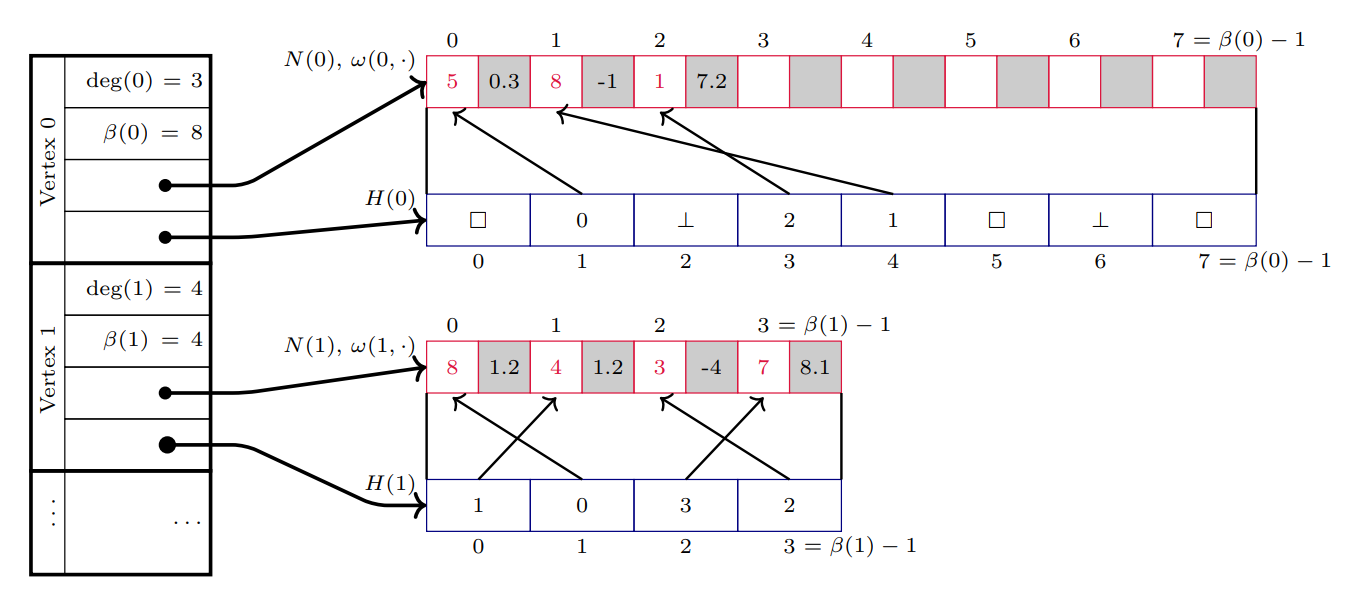
\includegraphics[width=1\textwidth]{images/layout_of_dhb.png}
\caption{Структура хеш-индексираних блокова суседства (DHB) \cite{vandergrinten_et_al:LIPIcs.SEA.2022.11}}
\label{fig:dhb_structure}
\end{figure}


\begin{example}
    Граф са слике \ref{fig:primer_dinamickog_grafa1} можемо једноставно представити DHB структуром. Како граф има четири чвора, потребна су нам четири блока суседства. Додавањем грана у граф ови блокови мењају своје величинe и садржај. На слици \ref{fig:dhb_jedna_grana} приказана је DHB структура након додавања гране $(1, 2)$, док на слици \ref{fig:dhb_sve_grane} видимо стање структуре након додвања свих преосталих грана. Приметимо да се величина блока првог чвора повећала са 2 на 4 након додавања гране $(1, 3)$, док су величине блокова осталих чворова остале непромењене.
\end{example}

\begin{figure}[htbp]
\centering
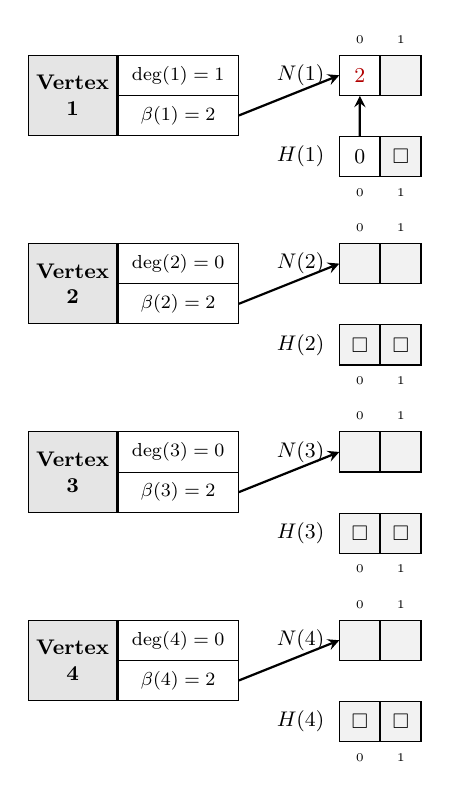
\begin{tikzpicture}[
    scale=0.85, every node/.style={transform shape},
    box/.style={draw, minimum height=0.6cm, minimum width=0.6cm, inner sep=0pt, align=center, font=\small},
    emptybox/.style={draw, fill=gray!10, minimum height=0.6cm, minimum width=0.6cm, inner sep=0pt, align=center, font=\small},
    headbox/.style={draw, minimum height=0.6cm, minimum width=1.8cm, inner sep=2pt, align=center, font=\footnotesize},
    titlebox/.style={draw, fill=gray!20, minimum height=1.2cm, minimum width=0.8cm, align=center, font=\bfseries\small},
    arrow/.style={->, >=stealth, thick}
]

% ==================== ЧВОР 1 ====================
\node[titlebox] (v1) {Vertex\\1};
\node[headbox, right=0cm of v1.north east, anchor=north west] (v1_deg) {$\deg(1) = 1$};
\node[headbox, right=0cm of v1.south east, anchor=south west] (v1_beta) {$\beta(1) = 2$};

% N(1) array
\node[box, right=1.5cm of v1_deg.east, anchor=west] (n1_0) {\textcolor{red!70!black}{2}};
\node[emptybox, right=0cm of n1_0] (n1_1) {};

\node[above=0.05cm of n1_0, font=\tiny] {0};
\node[above=0.05cm of n1_1, font=\tiny] {1};
\node[left=0.1cm of n1_0, font=\small] {$N(1)$};

% H(1) table
\node[box, below=0.6cm of n1_0] (h1_0) {0};
\node[emptybox, right=0cm of h1_0] (h1_1) {$\square$};

\node[below=0.05cm of h1_0, font=\tiny] {0};
\node[below=0.05cm of h1_1, font=\tiny] {1};
\node[left=0.1cm of h1_0, font=\small] {$H(1)$};

\draw[arrow] (v1_beta.east) -- (n1_0.west);
\draw[arrow] (h1_0.north) -- (n1_0.south);


% ==================== ЧВОР 2 ====================
\node[titlebox, below=1.6cm of v1.south west, anchor=north west] (v2) {Vertex\\2};
\node[headbox, right=0cm of v2.north east, anchor=north west] (v2_deg) {$\deg(2) = 0$};
\node[headbox, right=0cm of v2.south east, anchor=south west] (v2_beta) {$\beta(2) = 2$};

% N(2) array
\node[emptybox, right=1.5cm of v2_deg.east, anchor=west] (n2_0) {};
\node[emptybox, right=0cm of n2_0] (n2_1) {};

\node[above=0.05cm of n2_0, font=\tiny] {0};
\node[above=0.05cm of n2_1, font=\tiny] {1};
\node[left=0.1cm of n2_0, font=\small] {$N(2)$};

% H(2) table
\node[emptybox, below=0.6cm of n2_0] (h2_0) {$\square$};
\node[emptybox, right=0cm of h2_0] (h2_1) {$\square$};

\node[below=0.05cm of h2_0, font=\tiny] {0};
\node[below=0.05cm of h2_1, font=\tiny] {1};
\node[left=0.1cm of h2_0, font=\small] {$H(2)$};

\draw[arrow] (v2_beta.east) -- (n2_0.west);


% ==================== ЧВОР 3 ====================
\node[titlebox, below=1.6cm of v2.south west, anchor=north west] (v3) {Vertex\\3};
\node[headbox, right=0cm of v3.north east, anchor=north west] (v3_deg) {$\deg(3) = 0$};
\node[headbox, right=0cm of v3.south east, anchor=south west] (v3_beta) {$\beta(3) = 2$};

% N(3) array
\node[emptybox, right=1.5cm of v3_deg.east, anchor=west] (n3_0) {};
\node[emptybox, right=0cm of n3_0] (n3_1) {};

\node[above=0.05cm of n3_0, font=\tiny] {0};
\node[above=0.05cm of n3_1, font=\tiny] {1};
\node[left=0.1cm of n3_0, font=\small] {$N(3)$};

% H(3) table
\node[emptybox, below=0.6cm of n3_0] (h3_0) {$\square$};
\node[emptybox, right=0cm of h3_0] (h3_1) {$\square$};

\node[below=0.05cm of h3_0, font=\tiny] {0};
\node[below=0.05cm of h3_1, font=\tiny] {1};
\node[left=0.1cm of h3_0, font=\small] {$H(3)$};

\draw[arrow] (v3_beta.east) -- (n3_0.west);


% ==================== ЧВОР 4 ====================
\node[titlebox, below=1.6cm of v3.south west, anchor=north west] (v4) {Vertex\\4};
\node[headbox, right=0cm of v4.north east, anchor=north west] (v4_deg) {$\deg(4) = 0$};
\node[headbox, right=0cm of v4.south east, anchor=south west] (v4_beta) {$\beta(4) = 2$};

% N(4) array
\node[emptybox, right=1.5cm of v4_deg.east, anchor=west] (n4_0) {};
\node[emptybox, right=0cm of n4_0] (n4_1) {};

\node[above=0.05cm of n4_0, font=\tiny] {0};
\node[above=0.05cm of n4_1, font=\tiny] {1};
\node[left=0.1cm of n4_0, font=\small] {$N(4)$};

% H(4) table
\node[emptybox, below=0.6cm of n4_0] (h4_0) {$\square$};
\node[emptybox, right=0cm of h4_0] (h4_1) {$\square$};

\node[below=0.05cm of h4_0, font=\tiny] {0};
\node[below=0.05cm of h4_1, font=\tiny] {1};
\node[left=0.1cm of h4_0, font=\small] {$H(4)$};

\draw[arrow] (v4_beta.east) -- (n4_0.west);

\end{tikzpicture}
\caption{DHB структура за граф са слике \ref{fig:primer_dinamickog_grafa1} након додавања гране $(1, 2)$.}
\label{fig:dhb_jedna_grana}
\end{figure}

\begin{figure}[htbp]
\centering
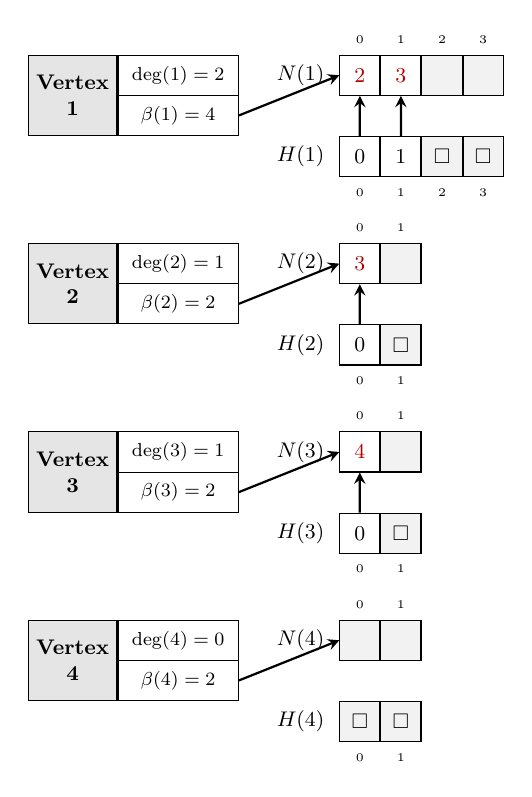
\begin{tikzpicture}[
    scale=0.85, every node/.style={transform shape},
    box/.style={draw, minimum height=0.6cm, minimum width=0.6cm, inner sep=0pt, align=center, font=\small},
    emptybox/.style={draw, fill=gray!10, minimum height=0.6cm, minimum width=0.6cm, inner sep=0pt, align=center, font=\small},
    headbox/.style={draw, minimum height=0.6cm, minimum width=1.8cm, inner sep=2pt, align=center, font=\footnotesize},
    titlebox/.style={draw, fill=gray!20, minimum height=1.2cm, minimum width=0.8cm, align=center, font=\bfseries\small},
    arrow/.style={->, >=stealth, thick}
]

% ==================== ЧВОР 1 ====================
\node[titlebox] (v1) {Vertex\\1};
\node[headbox, right=0cm of v1.north east, anchor=north west] (v1_deg) {$\deg(1) = 2$};
\node[headbox, right=0cm of v1.south east, anchor=south west] (v1_beta) {$\beta(1) = 4$};

% N(1) array
\node[box, right=1.5cm of v1_deg.east, anchor=west] (n1_0) {\textcolor{red!70!black}{2}};
\node[box, right=0cm of n1_0] (n1_1) {\textcolor{red!70!black}{3}};
\node[emptybox, right=0cm of n1_1] (n1_2) {};
\node[emptybox, right=0cm of n1_2] (n1_3) {};

\node[above=0.05cm of n1_0, font=\tiny] {0};
\node[above=0.05cm of n1_1, font=\tiny] {1};
\node[above=0.05cm of n1_2, font=\tiny] {2};
\node[above=0.05cm of n1_3, font=\tiny] {3};
\node[left=0.1cm of n1_0, font=\small] {$N(1)$};

% H(1) table
\node[box, below=0.6cm of n1_0] (h1_0) {0};
\node[box, right=0cm of h1_0] (h1_1) {1};
\node[emptybox, right=0cm of h1_1] (h1_2) {$\square$};
\node[emptybox, right=0cm of h1_2] (h1_3) {$\square$};

\node[below=0.05cm of h1_0, font=\tiny] {0};
\node[below=0.05cm of h1_1, font=\tiny] {1};
\node[below=0.05cm of h1_2, font=\tiny] {2};
\node[below=0.05cm of h1_3, font=\tiny] {3};
\node[left=0.1cm of h1_0, font=\small] {$H(1)$};

\draw[arrow] (v1_beta.east) -- (n1_0.west);
\draw[arrow] (h1_0.north) -- (n1_0.south);
\draw[arrow] (h1_1.north) -- (n1_1.south);


% ==================== ЧВОР 2 ====================
\node[titlebox, below=1.6cm of v1.south west, anchor=north west] (v2) {Vertex\\2};
\node[headbox, right=0cm of v2.north east, anchor=north west] (v2_deg) {$\deg(2) = 1$};
\node[headbox, right=0cm of v2.south east, anchor=south west] (v2_beta) {$\beta(2) = 2$};

% N(2) array
\node[box, right=1.5cm of v2_deg.east, anchor=west] (n2_0) {\textcolor{red!70!black}{3}};
\node[emptybox, right=0cm of n2_0] (n2_1) {};

\node[above=0.05cm of n2_0, font=\tiny] {0};
\node[above=0.05cm of n2_1, font=\tiny] {1};
\node[left=0.1cm of n2_0, font=\small] {$N(2)$};

% H(2) table
\node[box, below=0.6cm of n2_0] (h2_0) {0};
\node[emptybox, right=0cm of h2_0] (h2_1) {$\square$};

\node[below=0.05cm of h2_0, font=\tiny] {0};
\node[below=0.05cm of h2_1, font=\tiny] {1};
\node[left=0.1cm of h2_0, font=\small] {$H(2)$};

\draw[arrow] (v2_beta.east) -- (n2_0.west);
\draw[arrow] (h2_0.north) -- (n2_0.south);


% ==================== ЧВОР 3 ====================
\node[titlebox, below=1.6cm of v2.south west, anchor=north west] (v3) {Vertex\\3};
\node[headbox, right=0cm of v3.north east, anchor=north west] (v3_deg) {$\deg(3) = 1$};
\node[headbox, right=0cm of v3.south east, anchor=south west] (v3_beta) {$\beta(3) = 2$};

% N(3) array
\node[box, right=1.5cm of v3_deg.east, anchor=west] (n3_0) {\textcolor{red!70!black}{4}};
\node[emptybox, right=0cm of n3_0] (n3_1) {};

\node[above=0.05cm of n3_0, font=\tiny] {0};
\node[above=0.05cm of n3_1, font=\tiny] {1};
\node[left=0.1cm of n3_0, font=\small] {$N(3)$};

% H(3) table
\node[box, below=0.6cm of n3_0] (h3_0) {0};
\node[emptybox, right=0cm of h3_0] (h3_1) {$\square$};

\node[below=0.05cm of h3_0, font=\tiny] {0};
\node[below=0.05cm of h3_1, font=\tiny] {1};
\node[left=0.1cm of h3_0, font=\small] {$H(3)$};

\draw[arrow] (v3_beta.east) -- (n3_0.west);
\draw[arrow] (h3_0.north) -- (n3_0.south);


% ==================== ЧВОР 4 ====================
\node[titlebox, below=1.6cm of v3.south west, anchor=north west] (v4) {Vertex\\4};
\node[headbox, right=0cm of v4.north east, anchor=north west] (v4_deg) {$\deg(4) = 0$};
\node[headbox, right=0cm of v4.south east, anchor=south west] (v4_beta) {$\beta(4) = 2$};

% N(4) array (сва поља празна)
\node[emptybox, right=1.5cm of v4_deg.east, anchor=west] (n4_0) {};
\node[emptybox, right=0cm of n4_0] (n4_1) {};

\node[above=0.05cm of n4_0, font=\tiny] {0};
\node[above=0.05cm of n4_1, font=\tiny] {1};
\node[left=0.1cm of n4_0, font=\small] {$N(4)$};

% H(4) table (сва поља празна)
\node[emptybox, below=0.6cm of n4_0] (h4_0) {$\square$};
\node[emptybox, right=0cm of h4_0] (h4_1) {$\square$};

\node[below=0.05cm of h4_0, font=\tiny] {0};
\node[below=0.05cm of h4_1, font=\tiny] {1};
\node[left=0.1cm of h4_0, font=\small] {$H(4)$};

\draw[arrow] (v4_beta.east) -- (n4_0.west);

\end{tikzpicture}
\caption{DHB структура за граф са слике \ref{fig:primer_dinamickog_grafa1} након додавања свих грана.}
\label{fig:dhb_sve_grane}
\end{figure}


Декларација блока суседства у језику \texttt{C++} представљена је на листингу \ref{lst:vertex_interface}. Чвор је представљен класом \texttt{Vertex}, која садржи поља за идентификатор чвора, степен, величину блока суседа, низ суседа и хеш индекс. Класа такође садржи методе за управљање суседима, као што су додавање, уклањање и промена тежина грана, као и методе за итерацију кроз суседе.

Методе \texttt{AddNeighbor}, \texttt{RemoveNeighbor} и \texttt{ChangeWeight} омогућавају додавање, уклањање и измену тежина грана. Приликом додавања суседа, нови елемент се уписује на прву слободну позицију у низу суседа, док се хеш индекс ажурира тако да омогући константно време приступа, такође суседи се могу додавати уз одржавање сортираности по тежини гране. Уклањање суседа може се реализовати у два режима: без очувања редоследа, када се елемент замењује последњим елементом у низу (што омогућава сложеност $O(1)$), и са очувањем редоследа, када се врши померање елемената (што доводи до сложености $O(\deg(u))$).

Методе \texttt{IsNeighbor} и \texttt{GetWeight} користе хеш индекс за ефикасну проверу постојања суседа $v$ и приступ тежини гране између $u$ и $v$, са очекиваном временском сложеношћу $O(1)$. Итерација кроз суседе реализована је преко метода \texttt{NeighbourIterator} и \texttt{NeighbourEndIterator}, који омогућавају линеарни пролаз кроз првих $\deg(u)$ елемената низа.

Интерне методе \texttt{Find\allowbreak Slot}, \texttt{Find\allowbreak Insert\allowbreak Slot} и \texttt{Hash\allowbreak To\allowbreak Slot} реализују основне операције над хеш индексом, укључујући израчунавање почетне позиције и линеарно испитивање слотова приликом решавања колизија (енгл. \textit{linear probing}). Методе \texttt{RebuildHash\allowbreak Index} и \texttt{GrowAnd\allowbreak Rehash} служе за одржавање конзистентности и контролу фактора попуњености, при чему се у случају потребе врши проширивање блока и поновно хеширање елемената.

Додатне методе, као што су \texttt{SortEdges} и \texttt{RemapNeighborIds\allowbreak AfterVertex\allowbreak Removal}, омогућавају специфичне трансформације над вектором суседа, при чему је након ових операција неопходно поново изградити хеш индекс.

Детаљна анализа и опис механизама хеш индекса, укључујући стратегију разрешавања колизија и управљање слотовима, дата је у наредној подсекцији.

\begin{lstlisting}[style=thesiscpp, caption={Интерфејс класе \texttt{Vertex}}, label={lst:vertex_interface}]
class Vertex {
private:
    VertexID id;
    int degree;
    int beta;
    std::vector<Neighbor> neighbors;
    std::vector<HashEntry> hashes;

    int FindSlot(VertexID neighbor_id) const;
    int FindInsertSlot(VertexID neighbor_id, bool& already_present) const;
    int HashToSlot(VertexID neighbor_id) const;
    void RebuildHashIndex();
    void GrowAndRehash();

public:
    Vertex() = delete;
    explicit Vertex(VertexID id);

    VertexID Id() const;
    int Degree() const;
    int Beta() const;

    void AddNeighbor(VertexID neighbor_id, Weight weight = 1, bool keep_sorted_by_weight = false);
    void ChangeWeight(VertexID neighbor_id, Weight new_weight);
    void RemoveNeighbor(VertexID neighbor_id, bool preserve_order = false);
    bool IsNeighbor(VertexID neighbor_id) const;
    Weight GetWeight(VertexID neighbor_id) const;

    std::vector<Neighbor>::const_iterator NeighbourIterator() const;
    std::vector<Neighbor>::const_iterator NeighbourEndIterator() const;

    void SortEdges();
    void SetId(VertexID new_id);
    void RemapNeighborIdsAfterVertexRemoval(VertexID removed_vertex_id);
};
\end{lstlisting}

Граф је представљен класом \texttt{Graph}, која садржи низ чворова у графу и њихов број. Класа пружа методе за управљање чворовима и гранама, као што су додавање и уклањање чворова, додавање и уклањање грана, промена тежина грана, провера постојања грана и итерација кроз суседе. Све методе овог интерфејса представљају само омотач око метода класе \texttt{Vertex} са позивима за конкретан чвор. Интерфејс класе \texttt{Graph} представљен је на листингу \ref{lst:graph_interface}.

\begin{lstlisting}[style=thesiscpp, caption={Интерфејс класе \texttt{Graph}}, label={lst:graph_interface}]
class Graph {
public:
    explicit Graph(bool edges_sorted_by_weight = false) 
        : vertex_count(0), edges_sorted_by_weight(edges_sorted_by_weight) {}

    int VertexCount() const;
    VertexID AddVertex();
    void RemoveVertex(VertexID vertex_id);

    void AddEdge(VertexID vertex_id1, VertexID vertex_id2, Weight weight = 1);
    void RemoveEdge(VertexID vertex_id1, VertexID vertex_id2);
    Weight GetEdgeWeight(VertexID vertex_id1, VertexID vertex_id2) const;
    void UpdateEdgeWeight(VertexID vertex_id1, VertexID vertex_id2, Weight new_weight);

    bool AreNeighbors(VertexID vertex_id1, VertexID vertex_id2) const;
    std::vector<Vertex>::const_iterator VertexIterator() const;
    std::vector<Vertex>::const_iterator VertexEndIterator() const;
    std::vector<Neighbor>::const_iterator NeighbourIterator(VertexID vertex_id) const;
    std::vector<Neighbor>::const_iterator NeighbourEndIterator(VertexID vertex_id) const;

private:
    int vertex_count = 0;
    std::vector<Vertex> vertices;
    bool edges_sorted_by_weight = false;

};
\end{lstlisting}


\subsection{Хеш индекс}


Хеш индекс представља кључни механизам DHB структуре који омогућава ефикасну проверу постојања суседа и приступ њиховим позицијама у низу суседа. За сваки чвор $u$ дефинисан је хеш индекс $H(u)$ који садржи $\beta(u)$ елемената и реализован је као хеш табела са отвореним адресирањем\footnote{Хеш табела са отвореним адресирањем је структура у којој се сви елементи смештају директно у низ фиксне величине, а колизије се решавају испитивањем других позиција унутар истог низа (нпр. линеарним испитивањем). \cite{cormenIntroductionAlgorithms2009}} \cite{vandergrinten_et_al:LIPIcs.SEA.2022.11}.

За разлику од класичних хеш табела, хеш индекс не складишти директно податке о суседима, већ индексе у низу суседа $N(u)$. Сваки слот у хеш индексу може бити у једном од три стања \cite{vandergrinten_et_al:LIPIcs.SEA.2022.11}:
\begin{itemize}
    \item \texttt{EMPTY} - слот никада није био заузет,
    \item \texttt{OCCUPIED} - слот садржи важећи индекс у низу суседа,
    \item \texttt{DELETED} - слот је раније био заузет, али је елемент уклоњен (тзв. \emph{tombstone}).
\end{itemize}

Уколико је $H(u)[j]$ у стању \texttt{OCCUPIED}, онда тај елемент садржи индекс $i$ такав да важи $N(u)[i] = v$, где је $v$ сусед чвора $u$. Важи да је $i \in [0, \deg(u))$, чиме се обезбеђује конзистентност између хеш индекса и низа суседа \cite{vandergrinten_et_al:LIPIcs.SEA.2022.11}. 

На почетку су сви елементи хеш индекса постављени у стање \texttt{EMPTY}. Приликом додавања суседа, одговарајући слот се означава као \texttt{OCCUPIED} и у њега се уписује индекс новог суседа у низу $N(u)$. Приликом уклањања суседа, слот се не празни у потпуности, већ се поставља у стање \texttt{DELETED}, чиме се омогућава исправно функционисање линеарног испитивања \cite{vandergrinten_et_al:LIPIcs.SEA.2022.11}.

За одређивање почетне позиције користи се хеш функција $h : V \rightarrow \mathbb{N}$:
\[
j = h(v) \bmod \beta(u)
\]
Како је $\beta(u)$ степен двојке, ова операција се у имплементацији извршава као:
\[
j = h(v) \,\&\, (\beta(u) - 1)
\]

У случају колизије примењује се линеарно испитивање:
\[
j = (j + 1) \,\&\, (\beta(u) - 1)
\]

Овај поступак се понавља све док се не пронађе одговарајући слот \cite{vandergrinten_et_al:LIPIcs.SEA.2022.11}.

Претрага суседа $v$ помоћу хеш индекса чвора $u$ врши се тако што се креће од иницијалне позиције $j = h(v) \bmod \beta(u)$ и наставља линеарним испитивањем:
\begin{itemize}
    \item ако је $H(u)[j] = \texttt{EMPTY}$, претрага се завршава и $v$ није сусед,
    \item ако је $H(u)[j] = \texttt{OCCUPIED}$ и $N(u)[H(u)[j]] = v$, сусед је пронађен,
    \item у супротном, наставља се испитивање наредног слота.
\end{itemize}

Приликом уметања новог суседа $v$ најпре се врши претрага помоћу хеш индекса применом линеарног испитивања како би се проверило да ли сусед већ постоји. Током овог процеса памти се први слот у стању \texttt{DELETED}. Уколико се наиђе на слот у стању \texttt{EMPTY}, уметање се врши у тај слот или у раније пронађени \texttt{DELETED} слот. На овај начин се избегавају дупликати и омогућава ефикасно поновно коришћење слотова \cite{vandergrinten_et_al:LIPIcs.SEA.2022.11}.

Приликом брисања суседа, одговарајући слот у хеш индексу се означава као \texttt{DELETED}. Ово је неопходно како би се очувала исправност секвенци линеарног испитивања, јер би постављање слота у стање \texttt{EMPTY} могло прекинути претрагу за елементима који су уметнути касније у истој секвенци \cite{vandergrinten_et_al:LIPIcs.SEA.2022.11}.

Током времена може доћи до акумулације \texttt{DELETED} слотова, што негативно утиче на перформансе. Због тога се периодично врши реконструкција хеш индекса (\emph{rehashing}), при чему се сви важећи суседи чвора $u$ изнова убацују у празну хеш табелу. Ова операција има сложеност $O(\deg(u))$, али се дешава ретко и не утиче на амортизовану сложеност основних операција \cite{vandergrinten_et_al:LIPIcs.SEA.2022.11}.

У конкретној имплементацији, хеш индекс је представљен низом структура \texttt{HashEntry}, где сваки елемент садржи:
\begin{itemize}
    \item индекс у низу суседа,
    \item стање слота (\texttt{HashValue}).
\end{itemize}

Структура и енумерација приказани су на листингу \ref{lst:hash_index_interface}. Вредности \texttt{EMPTY} и \texttt{DELETED} реализоване су као специјалне негативне вредности, док \texttt{OCCUPIED} означава валидан унос. Ова репрезентација омогућава једноставну и ефикасну проверу стања слота током извршавања операција.

\begin{lstlisting}[style=thesiscpp, caption={Елементи хеш индекса}, label={lst:hash_index_interface}]
enum HashValue {
    OCCUPIED = 0,
    EMPTY = -1,
    DELETED = -2
};

struct HashEntry {
    unsigned index;
    HashValue hash_value;

    HashEntry() : index(-1), hash_value(EMPTY) {}
    HashEntry(unsigned index, HashValue hash_value) : index(index), hash_value(hash_value) {}
};
\end{lstlisting}


\section{Операције и сложености}

Како је граф представљен као низ хеш-индексираних блокова суседства, све операције над графом се своде на операције над појединачним блоковима. Интерфејс класе \texttt{Graph} представља једноставан омотач који делегира позиве одговарајућим методама класе \texttt{Vertex}. Због тога временске сложености операција над графом директно зависе од сложености операција над блоковима суседства.

Основне операције и њихове временске сложености су \cite{vandergrinten_et_al:LIPIcs.SEA.2022.11}:

\begin{itemize}
    \item \textit{Додавање чвора} се извршава у времену $O(1)$, јер подразумева иницијализацију новог блока суседства празним низом и хеш индексом.

    \item \textit{Уклањање чвора} има сложеност $O(\deg(u))$, где је $u$ чвор који се уклања, јер је потребно уклонити све гране инцидентне са њим и ажурирати информације о суседима тих чворова. У најгорем случају, када је чвор повезан са свим осталим чворовима, сложеност износи $O(|V|)$.

    \item \textit{Додавање гране} $(u, v)$ има амортизовану сложеност $O(1)$. Прво се путем хеш индекса проверава да ли се чвор $v$ већ јавља као сусед чвора $u$. Уколико то није случај, елемент се додаје на позицију $\deg(u)$ у низу $N(u)$, након чега се ажурира степен чвора $u$ и хеш индекс.  
    Уколико је потребно очувати редослед суседа (нпр. сортирано растуће по тежини гране) тада се сложеност ове операције мења, потребно је извршити померање елемената, што доводи до сложености $O(\deg(u))$.

    \item \textit{Уклањање гране} $(u, v)$ се извршава у амортизованом времену $O(1)$ уколико није потребно очувати редослед суседа, тако што се елемент проналази у хеш индексу и замењује последњим елементом у низу и затим уклања.  
    Уколико је потребно очувати редослед суседа, долази до померања елемената, што је сложености $O(\deg(u))$.

    \item \textit{Промена тежине гране} $(u, v)$ извршава се у амортизованом времену $O(1)$, јер се позиција суседа проналази преко хеш индекса, након чега се вредност директно ажурира.

    \item \textit{Провера постојања гране} $(u, v)$ извршава се у амортизованом времену $O(1)$ коришћењем хеш индекса.

    \item \textit{Итерација кроз суседе} чвора $u$ има сложеност $O(\deg(u))$, јер се врши линеарни пролаз кроз првих $\deg(u)$ елемената низа $N(u)$, без приступа хеш индексу.

    \item \textit{Промена редоследа суседа} (нпр. сортирање) врши се над низом $N(u)$. Сложеност ове операције зависи од конкретне трансформације која се примењује (нпр. $O(\deg(u)\log \deg(u))$ у случају сортирања). Након измене редоследа неопходно је поново изградити хеш индекс, што је операција сложености $O(\deg(u))$. Укупна сложеност је стога одређена сложеношћу примењене операције увећаном за трошак реконструкције хеш индекса.
\end{itemize}

% Implementacioni model i struktura

% ------------------------------------------------------------------------------
\chapter{Алгоритми}
% ------------------------------------------------------------------------------

\label{chp:algoritmi}
% Algoritmi

Алгоритми за рад са динамичким графовима имају кључну улогу у ефикасном одржавању и обради информација у графовима чија се структура мења током времена. За разлику од алгоритама над статичким графовима, алгоритми за динамичке графове често, поред саме алгоритамске процедуре, захтевају и употребу специјализованих структура података које омогућавају ефикасно ажурирање и одржавање информација од значаја. Због тога су овакви алгоритми по правилу сложенији и концептуално другачији у односу на класичне алгоритме над статичким графовима који се најчешће срећу у литератури.

У овом поглављу разматрају се проблеми одржавања информација о повезаности чворова и одржавања минималног разапињућег стабла у динамичким графовима. Ови проблеми имају значајну улогу у теорији графова и бројне примене у различитим областима, укључујући рачунарске мреже, друштвене мреже и биоинформатику.

\section{Динамичка повезаност}

Одржавање информације о повезаности чворова један је од најпроучаванијих проблема у области динамичких графова. Основни упит који је потребан за решавање овог проблема је \texttt{isConnected(u, v)}, који проверава да ли постоји пут између чворова \texttt{u} и \texttt{v} \cite{APPLICATIONS_OF_DYNAMIC_GRAPH}. У литератури се могу пронаћи ефикасне структуре података које омогућавају одржавање информација о повезаности у динамичким графовима, као што су \textit{Link-Cut Tree}, \textit{Euler Tour Tree} и \textit{Top Tree} \cite{APPLICATIONS_OF_DYNAMIC_GRAPH, holmPolylogarithmicDeterministicFullydynamic2001}. Ове структуре података омогућавају веома ефикасно одржавање информација о повезаности у динамичким графовима, али су по правилу сложене за имплементацију и најчешће специјализоване за одређену групу упита и операција над графом.

У овом поглављу биће предстваљено проширење DHB структуре података која омогућава одржавање информација о повезаности у инкременталним неусмереним динамичким графовима. Ово проширење засновано је на дисјунктним скуповима и омогућава ефикасно одржавање информација о компонентама повезаности у динамичким графовима. Упит \texttt{isConnected(u, v)} може се одговорити у константном времену. Додавање чворова има константу сложеност јер дирекнот користи DHB, док је додавање грана $O(\log n)$ због потребе за спајањем компоненти повезаности. Ово проширење DHB структуре података представља ефикасно решење за одржавање информација о повезаности у инкременталним неусмереним динамичким графовима.

\subsection{Имплементација}

\begin{lstlisting}[style=thesiscpp, caption={Интерфејс класе \texttt{DynamicConnectivityIncremental}}, label={lst:dc_interface}]
class DynamicConnectivityIncremental {
private:
    dg::Graph graph;
    std::vector<int> parent;
    std::vector<int> rank;

    int find(int x);
    void unite(int a, int b);

public:
    DynamicConnectivityIncremental() = default;

    int VertexCount() const;
    dg::VertexID AddVertex();
    
    void AddEdge(dg::VertexID vertex_id1, dg::VertexID vertex_id2, dg::Weight weight = 1);
    dg::Weight GetEdgeWeight(dg::VertexID vertex_id1, dg::VertexID vertex_id2) const;
    void UpdateEdgeWeight(dg::VertexID vertex_id1, dg::VertexID vertex_id2, dg::Weight new_weight);

    bool IsConnected(dg::VertexID vertex_id1, dg::VertexID vertex_id2);
};
\end{lstlisting}

\section{Динамичко минимално разапињуће стабло}

% Algoritmi

% ------------------------------------------------------------------------------
\chapter{Експериментална евалуација и резултати}
% ------------------------------------------------------------------------------

\label{chp:eksperimentalna_evaluacija_i_rezultati}
% Eksperimentala evaluacija i rezultati

Да би се верификовале теоријске анализе временске сложености и испитала практична ефикасност предложених динамичких алгоритама над DHB структуром, спроведена је експерименатална евалуација. Евалуација је усмерена на мерење времена извршавања основних операција ажурирања графа, као и специфичних упита који се извршавају над структуром података.

\section{Експериментално окружење}

Сва мерења извршена су у контролисаном хардверском и софтверском окружењу, са циљем да се обезбеде услови за репродуктивност експеримената и смањи утицај системских фактора на измерене резултате.

\subsection{Хардверско окружење:}

\begin{itemize}

\item \emph{Процесор:} Intel Core i5-1135G7 (11th Gen, Tiger Lake) са 4 физичка језгра и 8 логичких нити, базног такта $2.40\text{ GHz}$ и максималног \textit{Boost} такта до $4.20\text{ GHz}$.
\item \emph{Кеш меморија:} L1: $320\text{ KiB}$, L2: $5\text{ MiB}$, L3: $8\text{ MiB}$.
\item \emph{Оперативна меморија:} $16\text{ GB}$ DDR4.
\item \emph{Диск:} NVMe SSD Western Digital PC SN730 $512\text{ GB}$.

\end{itemize}

\subsection{Софтверско окружење и алати:}

\begin{itemize}

\item \emph{Оперативни систем:} Linux Mint 21.3 Virginia (64-bit).
\item \emph{Преводилац:} GCC 11.4.0.
\item \emph{Систем за изградњу:} CMake 3.16+ уз стандард C++17.
\item \emph{Оптимизација:} Сви извршни фајлови коришћени у евалуацији компајлирани су у \texttt{Release} режиму, уз оптимизацију кода помоћу заставице \texttt{-O3} и искључивање \texttt{assert} провера помоћу макроа \texttt{-DNDEBUG}. Ове опције су део глобалне CMake конфигурације пројекта.

\end{itemize}

\section{Начин мерења}

За потребе емпиријске евалуације перформанси имплементираних алгоритама, пројектовано је бенчмарк окружење у језику \texttt{C++} које помоћу \texttt{std::chrono} библиотеке мери време извршавања операција додавања грана и упита над тренутним стањем графа. Улазни подаци се псеудослучајно генеришу помоћу генератора са детерминистичким почетним стањем израчунатим на основу броја чворова и итерације ради обезбеђивања репродуктивности. 

Чворови се додају у граф у серијама од по $100$ чворова, а након сваке серије се врши псеудослучајно додавање грана између чворова. Мери се укупно време додвања свих грана у серији, након чега се израчунава просечно време по грани. Након тога извршава се $10.000$ упита зависно од одабраног алгоритма, а време извршавања се такође мери и израчунава просечно време по упиту. Овај процес понавља се 5 пута са различитим почетним стањем генератора, а коначан резултат се добија као просек свих појединачних мерења. Сви резултати се бележе у CSV фајл за накнадну анализу и визуализацију.

\section{Резултати}

На слици~\ref{fig:connectivity_plot} приказани су резултати перформанси инкременталног алгоритма за динамичку повезаност. Крива просечног времена додавања гране (\texttt{avg\_add\_edge\_ns}) показује благо логаритамско увећање са порастом броја чворова $|V|$, што је у потпуности сагласносно са теоријском сложеношћу $O(\log |V|)$ оствареном применом структуре дисјунктних подскупова. Са друге стране, крива за упит повезаности (\texttt{avg\_is\_connected\_ns}) је приближно константна током целог тестног опсега, чиме се практично потврђује амортизована сложеност $O(1)$ приликом испитивања припадности чворова истој компоненти повезаности.

\begin{figure}[h]
\centering
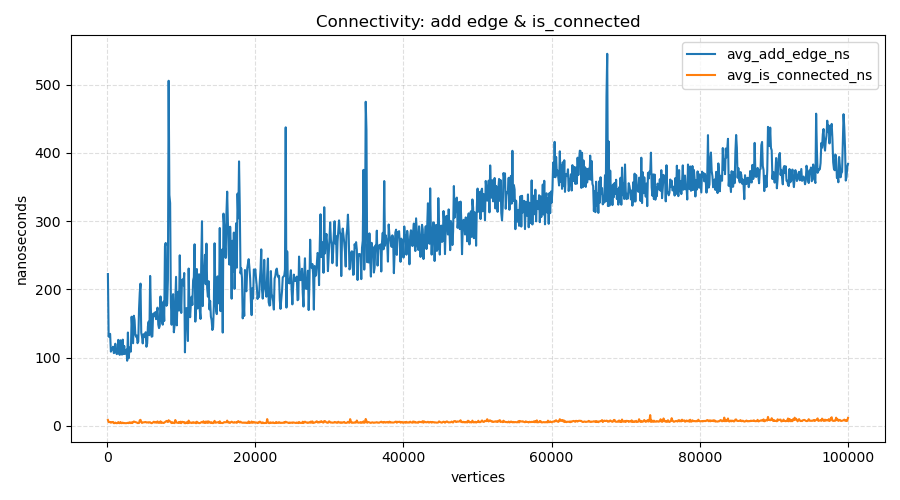
\includegraphics[width=1\textwidth]{images/connectivity_plot.png}
\caption{Резултати мерења за динамичку повезаност}
\label{fig:connectivity_plot}
\end{figure}

Резултати експерименталне евалуације за алгоритам одржавања динамичког минималног разапињућег стабла приказани су на слици~\ref{fig:mst_plot}. Време извршавања операције додавања гране која у себи укључује и реконструкције разапињуће шуме (\texttt{avg\_add\_edge\_ns}) показује приблично линеарни тренд раста у односу на број чворова $|V|$, што верно рефлектује изведену сложеност $O((|V|+|E|) \log |V|)$. Операција провере припадности гране минималном разапињућем стаблу (\texttt{avg\_is\_in\_mst\_ns}) показује стабилне и занемарљиве временске варијације, што потврђује ефикасност директног претраживања заснованог на хеш-индексирању у времену $O(1)$. 

\begin{figure}[h]
\centering
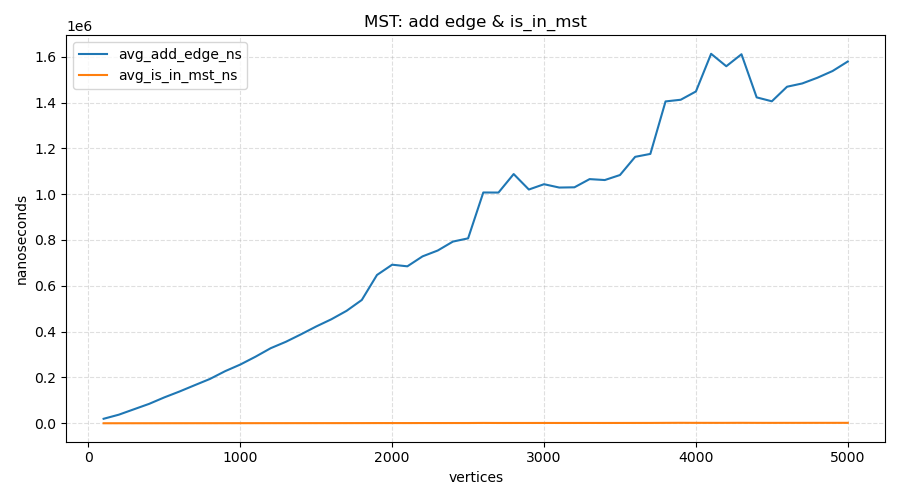
\includegraphics[width=1\textwidth]{images/mst_plot.png}
\caption{Резултати мерења за динамичко минимално разапињуће стабло}
\label{fig:mst_plot}
\end{figure}

На слици~\ref{fig:suitor_plot} приказано је временско понашање Суитор алгоритма. Мерења показују да време додавања гране (\texttt{avg\_add\_edge\_ns}) показује приближно линеарну зависност у односу на број чворова, што директно одговара теоријској сложености $O(|V|)$. Упит за проверу статуса упарености произвољног чвора (\texttt{avg\_is\_matched\_ns}) остаје на занемарљивој вредности током свих тестова, чиме се потврђује константна сложеност.

\begin{figure}[h]
\centering
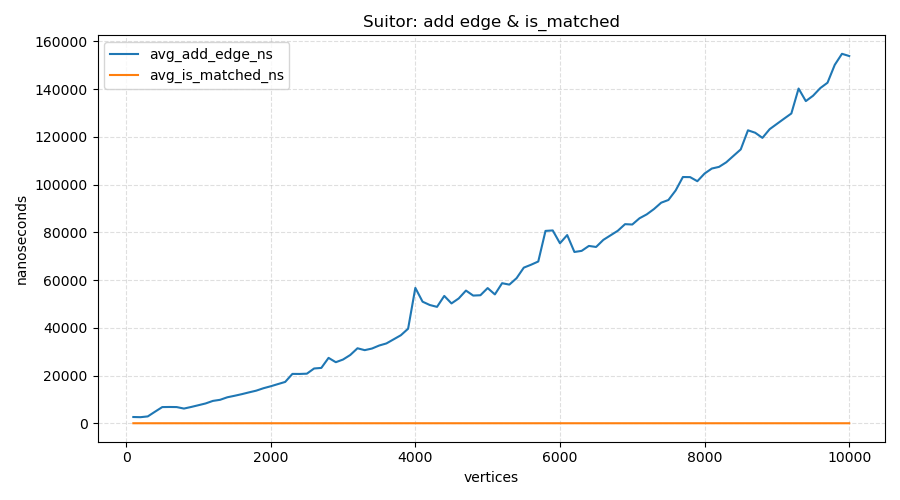
\includegraphics[width=1\textwidth]{images/suitor_plot.png}
\caption{Резултати мерења за Суитор алгоритам}
\label{fig:suitor_plot}
\end{figure}

% Eksperimentala evaluacija i rezultati

% ------------------------------------------------------------------------------
\chapter{Примене динамичких графова кроз примере}
% ------------------------------------------------------------------------------

\label{chp:primene}
% Primene dinamickih grafova

Динамички графови налазе широку примену у системима где се топологија мреже континуирано мења кроз време. Са порастом мрежне инфраструктуре, развојем науке и технологије потреба за ефикасним ажурирањима и одржавањем стања различитих мрежа у реалном времену је све више заступљена. 

У наредним секцијама биће представљене само неке од бројних примена динамичких графова како у науци тако и у индустрији, што додатно даје значај овој теми.

% Dinamicki grafovi 
\section{Анализа друштвених мрежа}

Једна од главних мрежа података су друштвене мреже. Друштвена мрежа састоји се од релација између различитих друштвених ентитета. Иако као друштвени ентитет најчешће видимо особе, друштвени ентитети такође су и групе људи, организације и било које друге групације које су повезане неким односима или интеракцијама између њих. Природно се овакве мреже моделују графовима, где су чворови друштвени ентитети, а гране представљају односе иземеђу њих~\cite{tabassumSocialNetworkAnalysis2018}. Друштвене мреже карактерише велики број честих промена па су динамички графови идеалне структуре за њихово моделовање~\cite{APPLICATIONS_OF_DYNAMIC_GRAPH}.

Над оваквим графовима можемо вршити разне анализе и испитивати односе међу ентитетима, пратити промене у тим односима и на основу тога доносити закључке о друштву и ентитетима у њему. На пример можемо испитивати који су ентитети најпознатији, најмање познати, који ентитеети повезују различите групе и слично. Ове особине лако се преносе на особине чворова у графу, рецимо уколико повезаност чворова представља релацију "познаје" и нека је та релација симетрична, тада је чвор највећег степена уједно и најпознатији ентитет у друштву. 

Једно својство специфично за друштвене мреже је тенденција креирања заједница (енгл. \textit{communitygraph}). У контексту графова заједнице видимо као подграфове у којима су чворови густо повезани, а шворови из различитих подграфова ретко повезани. На слици \ref{fig:community_graph} можемо видети пример друштва са дванаест ентитета и три заједнице~\cite{tabassumSocialNetworkAnalysis2018}.


\begin{figure}[ht]
\centering
\begingroup
\shorthandoff{"}
\digraph[scale=0.6]{communitygraph}{
    node [shape=circle];
    edge [dir=none];

    subgraph cluster_A {
        style=filled;
        color=lightgrey;

        A1 -> A3;
        A2 -> A3;
        A3 -> A4;
        A4 -> A1;
        A1 -> A3;
    }

    subgraph cluster_B {
        style=filled;
        color=lightblue;
        B1 -> B2;
        B2 -> B3;
        B3 -> B4;
        B1 -> B4;
        B2 -> B4;
    }

    subgraph cluster_C {
        style=filled;
        color=lightyellow;
        C1 -> C2;
        C2 -> C3;
        C4 -> C1;
        C2 -> C4;
    } 

    A4 -> B1;
    B4 -> C2 [constraint=false];
    A2 -> C3 [constraint=false];
}
\endgroup
\caption{Друштво са 12 ентитета и 3 заједнице}
\label{fig:community_graph}
\end{figure}

\section{Интернет и Google PageRank}

Развојем интернета број страница и хиперлинкова између њих је растао великом брзином. Структура која се користи за чување и анализу ових података зове се Веб граф (енгл. \textit{The Web graph}). Веб граф представља усмерени граф чији су чворови интернет странице, а два чвора $u$ и $v$ су повезана граном уколико страница $u$ садржи хиперлинк на страницу $v$. Веб граф је огроман објекат, тренутно садржи преко 3 милијарде чворова повезаних са преко 50 милијарди грана~\cite{boldiWebgraphFrameworkCompression2004}. Како се у времену интернета број страница и хиперлинкови између њих мењају свакодневно динамички графови представљају погодан избор за ефикасно чување и анализу ових података. 

\subsection{Google PageRank}

PageRank је алгоритам за анализу линкова који се заснива на концепту централности сопствених вектора (\textit{eigenvector centrality}). Овај алгоритам користи интернет претраживач Google како би рангирао веб странице на основу вредности информација које оне носе, тако да се највредније странице приказују на самом врху резултата претраге. Основна идеја алгоритма јесте да се информације на вебу могу рангирати према популарности линкова. Што више веб страница показује на одређену страницу, то је она популарнија. Међутим, у овом процесу вредновања није релевантан само број линкова (односно степен чвора), већ и значај самих страница које упућују на њу. Стога PageRank мери релативни значај скупа веб страница не само на основу квантитета, већ пре свега на основу квалитета њихових линкова~\cite{boldiWebgraphFrameworkCompression2004}. Алгоритам PageRank један је од најпопуларнијих алгоритама на свету стога је вредно поменути га, али за потребе овог рада нећемо га детаљније објашњавати.

% Dynamic connectivity incremental
\section{Ширење заразних болести}

Болести као што су прехлада, грип, велике богиње или SARS, преносе се ваздухом између две особе које у затвореном простору проведу довољно времена заједно. То значи да можемо претпоставити да ће већина инфекција настати на локацијама као што су канцеларије, тржни центри, јавни превоз и слично~\cite{toroczkaiProximityNetworksEpidemics2007}. Већина стандардних математичких модела за ширење заразних болести користи диференцијалне једначине засноване на претпоставкама о униформном мешању или насумичне моделе који описују процес контакта~\cite{eubankModellingDiseaseOutbreaks2004}. Ипак, праћењем кретања људи можемо генерисати контактну мрежу, односно бипартитни граф $G_{PL}$ који се састоји од две врсте чворова: особа ($P$) и локација ($L$)~\cite{toroczkaiProximityNetworksEpidemics2007, eubankModellingDiseaseOutbreaks2004}. 

Уколико је особа $p$ посетила локацију $l$, у овом бипартитном графу постоји грана између чворова $p$ и $l$. Чворови могу бити означени одговарајућим демографским или географским подацима, док се гранама могу доделити ознаке са временом доласка и одласка. Из оваквог бипартитног графа природно се добијају две пројекције повезивањем свих парова чворова који се у бипартитном графу налазе на растојању два. Као резултат добијају се два засебна графа: граф особа $G_P$ и граф локација $G_L$. У графу особа $G_P$, гране су означене временским интервалима током којих су се особе налазиле на истој локацији. Ради једноставности, често се посматра статичка пројекција $\hat{G}_P$, која се добија занемаривањем временских ознака~\cite{eubankModellingDiseaseOutbreaks2004}.

Како се људи крећу и мењају своје локације, тако се и контактна мрежа мења. Стога је динамички граф погодна структура за моделовање оваквих мрежа. С обзиром на то да се у оваквим мрежама чворови и гране могу само додавати, јер једном остварен контакт у историји преноса не може бити избрисан, прецизније можемо рећи да је контактна мрежа инкрементални динамички граф.

У оваквом систему можемо искористити алгоритам динамичке повезаности да бисмо пратили ширење инфекције. Користећи пројекцију графа $G_P$ можемо пратити како се инфекција шири кроз популацију, док коришћењем пројекције $G_L$ пратимо угроженост самих локација. Проверу да ли је инфекција потенцијално достигла одређену особу или локацију вршимо једноставним упитом \texttt{IsConnected}, испитујући да ли су иницијално заражена особа и посматрана особа повезане у графу $G_P$. Сличну проверу можемо вршити и за локације у графу $G_L$.


\section{Протеин протеин интеракције}

\cite{zhangConstructionDynamicProbabilistic2016}

% MST
\section{3D реконструкција слика}

% Suitor Matching
\section{Алокација радних оптерећења у cloud инфраструктури}
\section{Препоручивање}



% Primene dinamickih grafova

% ------------------------------------------------------------------------------
\chapter{Закључак}
% ------------------------------------------------------------------------------

\label{chp:zakljucak}
% Zakljucak

У овом мастер раду разматрана је проблематика ефикасне обраде и управљања динамичким графовима, који представљају кључни математички и рачунарски модел за репрезентацију савремених комплексних система склонх променама током времена. Традиционални приступи, који се ослањају на анализаторе статичких графова или периодично поновно израчунавање свих својстава система, показују озбиљна ограничења у погледу временске и просторне сложености када се примене на окружења са високом фреквенцијом ажурирања.

Кроз детаљну анализу постојећих имплементационих модела из литературе, у раду је истакнута потреба за структуром података која балансира између брзине структурних модификација и ефикасности аналитичких пролаза кроз суседства чворова. Тежиште рада стављено је на структуру хеш-индексираних блокова суседства. DHB структура кроз комбинацију секвенцијалног смештања суседа у контигуалне блокове и хеш-индекса са отвореним адресирањем успешно спаја добре особине низова (константан индексни приступ, просторна локалност, ефикасна итерација) и хеш-табела (брза провера постојања гране и промена тежине у $O(1)$ времену).

Главни истраживачки и практични допринос овог рада огледа се у реализацији C++ библиотеке засноване на DHB структури и њеној успешној адаптацији за решавање фундаменталних графовских проблема у динамичким условима:
\begin{itemize}
    \item \textit{Инкрементална динамичка повезаност:} Интеграцијом DHB структуре са помоћном структуром дисјунктних подскупова омогућено је праћење компоненти повезаности и одговарање на упите о повезаности чворова у амортизованом готово константном времену, уз задржавање ефикасних инкременталних измена.
    \item \textit{Динамичко минимално разапињуће стабло:} Искоришћена је флексибилност DHB структуре у одржавању произвољног и сортираног поретка суседа. Применом мин-хипа над унапред сортираним блоковима суседства елиминисана је потреба за скупим глобалним сортирањем свих грана графа, чиме је постигнута значајно боља асимптотска ефикасност одржавања минималне разапињуће шуме након сваке промене тежина или структуре.
    \item \textit{Динамичко максимално тежинско упаривање:} Приказано је како одржавање опадајућег поретка тежина у блоковима суседства директно погодује похлепним алгоритмима апроксимације. DHB омогућава дохватање гране са највећом тежином у $O(1)$ времену преко реверзних итератора, што омогућава брзу евалуацију понуда у Суитор алгоритму и ефикасно одржавање $1/2$-максималног тежинског упаривања.
\end{itemize}

Иако разматрани алгоритми нису имплементирани потпуно динамички, већ се одређена количина информација израчунава изнова, примарни фокус био је на демонстрацији особина DHB структуре у погледу ефикасности и могућности прилагођавања динамичким променама. Важно је нагласити да се DHB структура не може користити као потпуно самостално решење за све динамичке алгоритме, нити сама по себи покрива све функције неопходне за различите примене. Уместо тога, она служи као изузетно ефикасно складиште основних градивних елемената графа. Тиме је показано да DHB структура представља солидну основу за развој потпуно динамичких алгоритама који би омогућили одржавање својстава графа у присутству и инкременталних и декременталних операција.

Поред теоријске и имплементационе анализе, у раду је кроз репрезентативне примере показано да динамички графови нису само апстрактни концепт, већ да постоји реална и све већа потреба за њиховом применом, како у научним тако и у индустријским окружењима.

Као главни правци будућег истраживања и надградње овог рада истичу се проширење DHB структуре ради подршке за потпуно динамичке алгоритме са ефикасним ажурирањима, као и имплементација напредних паралелних и дистрибуираних варијанти ове структуре. Такође, значајан фокус будућег рада може бити на даљој оптимизацији управљања меморијом приликом фреквентних операција реалокације и поновног хеширања, применици овог модела у динамичком машинском учењу над графовима (енгл. \textit{Dynamic Graph Neural Networks}), као и у развоју графовских база података са високом фреквенцијом измена где динамичке структуре играју кључну улогу у ефикасном управљању и анализи података.

% Zakljucak

% ------------------------------------------------------------------------------
% Literatura
% ------------------------------------------------------------------------------
\literatura

% ==============================================================================
% Završni deo teze i prilozi
\backmatter
% ==============================================================================

% ------------------------------------------------------------------------------
% Biografija kandidata
\begin{biografija}
\textbf{Марко Лазаревић} рођен је 4. априла 2002. године у Фочи, Босна и Херцеговина. Средњу Техничку школу у Чачку завршио је 2021. године, када уписује Математички факултет Универзитета у Београду. Основне академске студије на модулу Информатика завршава 2025. године са просечном оценом 9,35, након чега на истом факултету уписује и мастер студије на истоименом модулу. У периоду од јула до октобра 2025. године обављао је стручну праксу у компанији \textit{Nutanix} у Београду. Од новембра 2025. године запослен је у истој компанији на позицији софтверског инжењера, где се бави развојем софтвера и савременим дистрибуираним системима.
\end{biografija}
% ------------------------------------------------------------------------------

\end{document} 